\documentclass{minimal}

\usepackage[compat=1.1.0]{tikz-feynman}


\tikzfeynmanset{ fermion/.style = {
   decoration={
     markings,
     mark=at position 0.5
          with {\arrow[xshift=.7mm]{latex[width=1mm,length=1mm]}}
     },
   postaction=decorate
   }
}

\begin{document}
\begin{equation}
\mathcal{M} =
    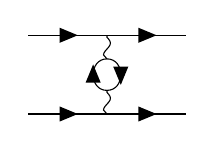
\begin{tikzpicture}[baseline=(c)]
        \begin{feynman}
            \vertex (a1) at (0, 0);
            \vertex (c1) at (2, 0);
            \vertex (a2) at (0, -1);
            \vertex (c2) at (2, -1);
            \vertex (x) at (1, 0);
            \vertex (l1) at (1, -.3);
            \vertex (c) at (1, -.5);
            \vertex (l2) at (1, -.7);
            \vertex (y) at (1, -1);
            \diagram*{
                {[edges=fermion]
                (a1) -- (x) -- (c1),
                (a2) -- (y) -- (c2),
                (l1) --[half left, looseness=1.5] (l2) --[half left, looseness=1.5] (l1),
                },
                {[edges=photon]
                (x) -- (l1),
                (l2) -- (y)
                }
            };
        \end{feynman}
    \end{tikzpicture}
\end{equation}
\begin{equation}
    \mathcal M =
    \feynmandiagram[small, baseline=(a)]{
        a [dot] --[fermion, out=130, in=230, min distance=2cm, looseness=1] a,
        a --[fermion, out=50, in=310, min distance=2cm, looseness=2] a,
    };
    \feynmandiagram[small, baseline=(a), horizontal=a to b]{
        a [dot] --[fermion, out=130, in=230, min distance=2cm, looseness=1] a,
        a -- [fermion, quarter right] b [dot] -- [fermion, quarter right] a,
        b --[fermion, out=50, in=310, min distance=2cm] b,
    };
\end{equation}
\end{document}